\chapter{A geometrical description of vortex variability}
\label{cha:moments}

% To Do: 
% - Discussion of sensitivity of the clustering algorithm
% - Description of dripping paint plot
% - Significance for dripping paint plot
% - CP07 and M13 events in table (or maybe disagreeing events highlighed
%   - plot disagreeing events seperately to check 


\section{Introduction}
Stratospheric sudden warmings (SSWs) are extreme events in which the strong
westerly winds that usually dominate the winter polar stratosphere become highly
disturbed (here, for reasons outlined below, we use the term SSW to encompass a
wider range of variability than its traditional definition). These events lead
to the mixing of mid-latitude air into the polar vortex region, causing an
increase in temperatures by several tens of kelvin over the course of a few
days. Traditional methods to identify stratospheric sudden warmings (SSWs) have
relied on either zonal-mean \citep{Andrews1987} or annular mode
\citep{Baldwin2001a} diagnostics. Neither method explicitly deals with the
inherent zonal asymmetry in vortex variability. In particular, SSWs are observed
to occur in one of two manners: displaced vortex events, where the vortex moves
far from the pole, and split vortex events, where the vortex separates into two
`child' vortices. These two types have a very different spatial structure and
evolution timescale \citep{Matthewman2009}. Displaced and split vortex events
are predominantly associated with vertically propagating Rossby waves of
wavenumber 1 and 2 respectively, and many previous studies have classified SSWs
based on wavenumber \citep[e.g.][]{Nakagawa2006}. However, this method does not
provide a description of the location of the polar vortex itself, which
theoretical arguments suggest may be important for understanding
stratosphere-troposphere coupling \citep{Ambaum2002}. In an improvement to these
traditional SSW definitions, \citet{Charlton2007a} (hereafter CP07) introduced a
classification in which a split vortex event is identified when two vortices
with a circulation ratio of 2:1 or higher are present, and all other SSWs are
automatically classed as displaced vortex events. However, they maintained the
traditional SSW identification which requires there to be a reversal of the
zonal-mean zonal wind at 10~hPa and $60^{\circ}$N.

An increased understanding of stratospheric variability can be gained by using
vortex-centric diagnostics, such as two-dimensional (2D) vortex moments
\citep{Waugh1997, Waugh1999, Mitchell2011, Mitchell2011a}, which provide a
geometrical description of the vortex and have no reliance on zonal-mean
properties. Using a classification based on these diagnostics,
\citet{Mitchell2013} (hereafter M13) identified a greater number of SSWs than
CP07. This is primarily because they did not use a zonal mean threshold
criterion. Importantly, M13 also demonstrated that split vortex events
penetrated deep into the troposphere and resulted in significant surface
anomalies, while anomalies associated with displaced vortex events do not
descend far below the tropopause. Their result supported a similar conclusion by
\citet{Nakagawa2006}, who found that the impact of events associated with an
enhanced upward flux of wavenumber-2 planetary waves was more likely to reach
the surface. These results underline the need to correctly identify the precise
type of SSW, in order to understand stratosphere-troposphere coupling within
climate models.

Distinguishing between displaced and split vortex events using the method of M13
requires the use of potential vorticity (PV), which is not commonly output by
climate models. For this reason, previous attempts to apply PV-based techniques
in a multi-model study have led to the majority of models being excluded
\citep{Mitchell2012a}. Furthermore, their method used a hierarchical clustering
technique \citep{Hannachi2010}, which is very sensitive to the exact shape of
the distribution of vortex variability, so is unsuitable for application to a
range of models with different climatologies. In this chapter, we develop an
improved method which; (a), is based on the geometry of the vortex, but requires
only the 10~hPa geopotential height; and (b), identifies events using a simple
threshold instead of a clustering technique. We apply this new method to the
ERA-40 and ERA-Interim reanalysis datasets and demonstrate that the method
captures a similar number of events which are in good agreement with, and at
least as extreme as, those of M13.


\section{The $Z_{10}$ method}
\subsection{Vortex geometry calculation}

Northern Hemisphere winter daily-mean data for December-March (DJFM) were
employed. The European Centre for Medium-Range Weather Forecasts (ECMWF) ERA-40
dataset \citep{Uppala2005} is used from 1958-1979 and ERA-Interim
\citep{Dee2011} from 1979-2009. The geometry of the vortex is described in terms
of the latitude of the centre of the vortex (centroid latitude) and aspect ratio
(a measure of how stretched the vortex
is).

The method calculates the 2D vortex moment of order $a+b$, defined in Cartesian
coordinates as
 \begin{equation}
 \mu_{ab} = \int \!\!\! \int_{S}[X(x,y) - \bar{X}]x^{a}y^{b}\mathrm{d}x\mathrm{d}y \, , 
 \label{eqn1}
 \end{equation}
 where $\bar{X}$ is a single contour of PV or geopotential height, representing
 the vortex edge. The value of this contour is chosen to match that of the
 10~hPa geopotential height ($Z_{10}$) or 850~K PV (PV$_{850}$) DJFM zonal-mean
 at 60$^{\circ}$N (however, the results are not sensitive to the exact choice of
 contour between about 50$^{\circ}$-70$^{\circ}$N). Following the method of
 \citet{Matthewman2009} (to which readers are referred for technical details),
 Equation \ref{eqn1} allows for the explicit calculation of the centroid
 latitude and aspect ratio on a particular pressure level or isentropic
 surface. Other moment diagnostics can be extracted, such as vortex area and
 kurtosis, but these were not found necessary for identifying split and
 displaced vortex events, and are therefore omitted from the
 analysis. %Matthewman??

 \begin{figure}
 \centering 
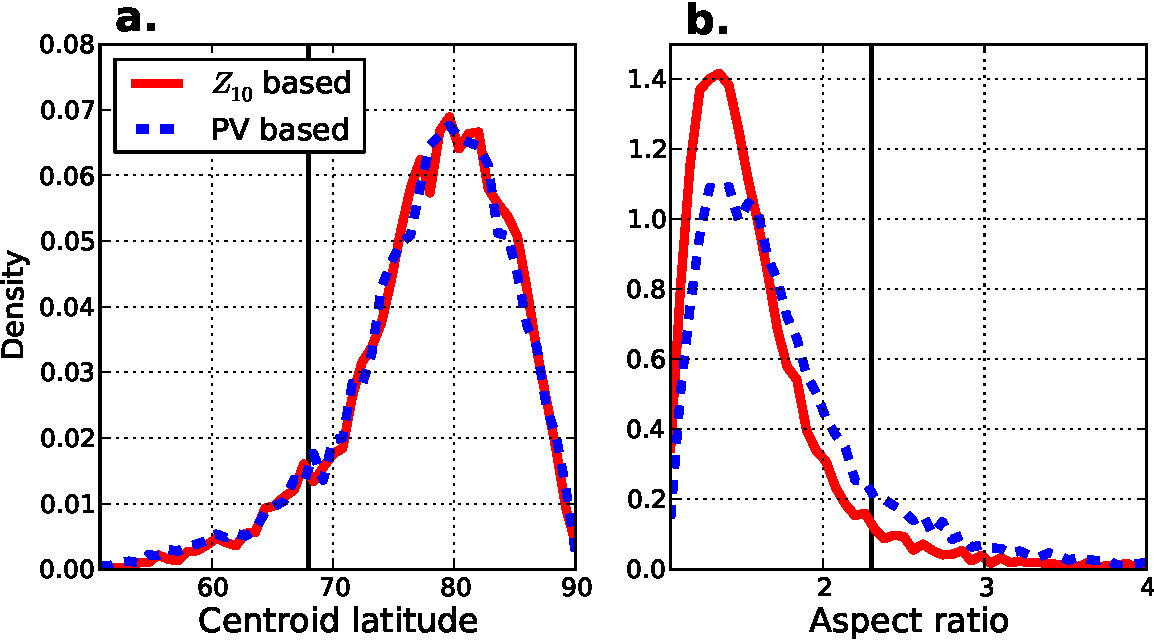
\includegraphics[width=\textwidth]{figures/chapter-moments/moments_distribution_crop.pdf}
\caption[Distributions of $Z_{10}$ and PV-based moment
diagnostics.]{Distributions of the December-March centroid latitude (a) and
  aspect ratio (b), of the Northern Hemisphere stratospheric polar vortex over
  1958-2009. Diagnostics are calculated from geopotential height at 10~hPa
  ($Z_{10}$) and potential vorticity at 850~K (PV). Thresholds of 66$^{\circ}$N
  in centroid latitude and 2.4 in aspect ratio are used to define events, and
  are indicated by the black vertical lines.}
 \label{Fig1}#
 \end{figure}
 Figure \ref{Fig1} compares the distribution of aspect ratio and centroid
 latitude, calculated using daily PV$_{850}$ and $Z_{10}$. The centroid latitude
 distributions are almost identical, with a peak around $80^{\circ}$N. The
 aspect ratio distributions have a similar shape, with a peak at about 1.3, but
 the PV based diagnostic has a larger tail. This is to be expected, since the PV
 field contains more small-scale, filamentary structures than geopotential
 height. Neither distribution shows bi-modality, suggesting that the application
 of clustering techniques, as in \citet{K.Coughlin2009} and
 \citet{Hannachi2010}, may be inappropriate. As well as having similar
 distributions, the timeseries of the PV and geopotential height derived
 diagnostics (not shown) are well correlated, with correlation coefficients of
 0.9 for centroid latitude and 0.6 for aspect ratio.



\subsection{Event definition}

In order to identify displaced and split vortex events, a threshold criterion is
introduced and applied to the geopotential height derived diagnostics. A
displaced vortex event requires the centroid latitude to remain equatorward of
66$^{\circ}$N for 7 days or more. A split vortex event requires the aspect ratio
to remain higher than 2.4 for 7 days or more. These thresholds are indicated in
Figure \ref{Fig1}, and were selected to give a similar frequency of displacement
and splitting events as M13. This choice is somewhat subjective, but the results
presented below are not sensitive to the exact choice of threshold. There were
no occasions on which both criteria were met simultaneously. The onset date is
defined as the day that the appropriate threshold is first exceeded, and to
ensure that no events are counted twice, the events are required to be spaced at
least 30 days apart, chosen to reflect radiative timescales in the lower
stratosphere \citep{Newman1997}.  \citet{Mitchell2011} found that the aspect
ratio and centroid latitude follow an extreme value distribution \citep{Cole}
and we note that both thresholds chosen here lie beyond the extreme value
thresholds of their respective distributions. Using this method, 17 displaced
and 18 split vortex events (listed in Table 2.1) are identified over the 52
winters, an average of 7 per decade. These events are all mid-winter events --
the DJFM data were used explicitly to avoid counting final warmings. This
frequency lies between the values of CP07 (6/decade) and M13 (8/decade).

% To Do: Change this figure to a horizontal one
 \begin{figure}
 \centering
 \noindent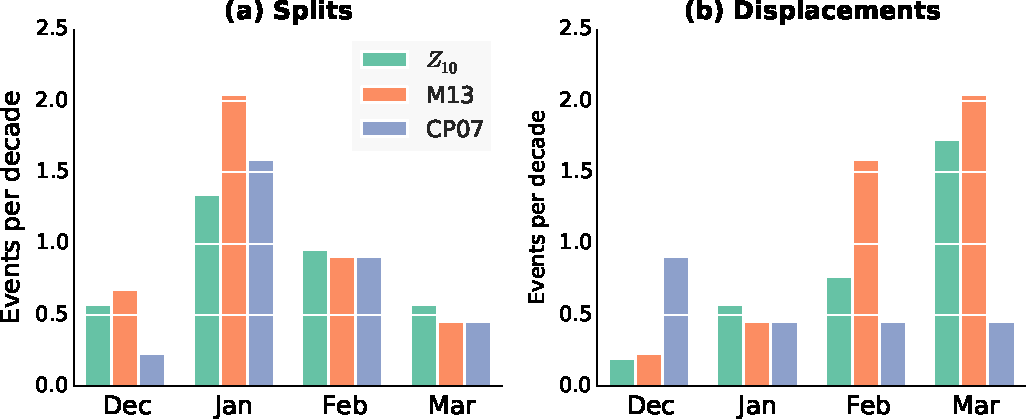
\includegraphics[width=\textwidth]{figures/chapter-moments/splits_displacements_histogram.pdf}
 \caption[Seasonal distribution of dispalaced and split vortex
 events.]{Histogram of the seasonal distribution of displaced and split vortex
   events, form the $Z_{10}$ method, M13 and CP07.}
 \label{Fig2}
 \end{figure}
 There are significant differences in the seasonal distribution of displaced and
 split vortex events, as shown in Figure \ref{Fig2}. Split vortex events are
 more frequent in early-mid winter, with a peak in January, while displaced
 vortex events are skewed towards late winter. Figure \ref{Fig2} also shows the
 seasonal distribution of displaced and split vortex events from CP07 and
 M13. The shape of the distribution agrees well with the seasonal distribution
 found by M13 for both types of event. However, there is less similarity with
 the CP07 distribution of displaced vortex events (Figure \ref{Fig2}b). CP07
 indicates an approximately flat distribution throughout winter, and many fewer
 displaced vortex events overall. It should be noted that the seasonal
 distribution of displaced and split vortex events from the moment based methods
 does not arise from the underlying climatology of centroid latitude or aspect
 ratio, which remains approximately constant throughout winter
 \citep{Mitchell2011}.

\begin{table}
\begin{centering}
    \begin{tabular}{|l|l|l|l|}  \hline
    No. & Event onset & Event type & $\Delta \mathrm{T}_{10}$ (K) \\ \hline
    1*  & 1961-3-9    & D          & 10.2        \\
    2*  & 1962-1-30   & S          & 1.9         \\
    3*  & 1962-3-7    & S          & -1.0        \\
    4*  & 1964-3-15   & D          & 11.9        \\
    5   & 1966-2-26   & D          & 2.5         \\
    6   & 1967-12-29  & S          & 13.0        \\
    7   & 1970-1-5    & S          & 8.5         \\
    8   & 1971-1-15   & S          & 10.8        \\
    9*  & 1972-2-4    & S          & -1.6        \\
    10  & 1973-2-4    & S          & 7.3         \\
    11* & 1974-3-12   & D          & 5.3         \\
    12* & 1975-3-16   & D          & 7.6         \\
    13* & 1976-3-31   & D          & 8.2         \\
    14  & 1977-1-7    & S          & 7.6         \\
    15* & 1978-3-25   & D          & 2.5         \\
    16  & 1979-2-18   & S          & 5.6         \\
    17  & 1984-2-25   & D          & 11.6        \\
    18  & 1984-12-25  & S          & 15.0        \\
    19* & 1986-1-7    & S          & 3.4         \\
    20* & 1986-3-21   & D          & 9.1         \\
    21  & 1987-1-20   & D          & 8.3         \\
    22  & 1987-12-10  & S          & 9.8         \\
    23* & 1992-3-22   & D          & 7.6         \\
    24* & 1995-2-2    & D          & 5.6         \\
    25  & 1998-12-15  & D          & 8.2         \\
    26  & 1999-2-24   & S          & 6.6         \\
    27  & 2001-2-7    & S          & 5.2         \\
    28* & 2001-3-15   & S          & -6.8        \\
    29* & 2002-3-21   & S          & -1.5        \\
    30  & 2003-1-17   & S          & 6.1         \\
    31  & 2004-1-2    & D          & 5.8         \\
    32* & 2005-3-11   & D          & 3.1         \\
    33  & 2006-1-17   & D          & 4.2         \\
    34  & 2008-2-18   & D          & 4.6         \\
    35  & 2009-1-18   & S          & 13.2        \\ \hline
    \end{tabular}
    \caption{A summary table of displaced (D) and split (S) vortex events,
      identified using the Z10 method for data from 1958-2009.
      $\Delta \mathrm{T}_{10}$ represents the mean area-weighted
      $50^{\circ}$-$90^{\circ}$N cap temperature anomaly at 10 hPa calculated 5
      days either side of the event onset date. Stars represent those numbers
      that do not coincide (within 10 days) with events defined by CP07.}
\end{centering}
\label{tab:events}
\end{table}

\section{Analysis}

To evaluate how well the new method captures displaced and split vortex events,
Figure \ref{Fig3} shows composites of PV in the mid-stratosphere (850~K)
following their onset dates. These are averaged over the 5 days following the
onset date for split events and 7 days for displaced events (these averaging
periods reflect the different timescales of the events). The composites are
compared with the corresponding composites following the events identified by
M13 and CP07. For the split vortex events, the $Z_{10}$ method clearly shows two
separated vortices, one centred over Canada and the other over Siberia. This
characteristic direction reflects the climatological wave-2 pattern at this
altitude. For the M13 events the split vortex composite shows the vortex
stretched across the same $90^{\circ}$W-$90^{\circ}$E line, although not as
clearly split, while the composite for the CP07 events looks very
different. This has a weak vortex centred over Canada, with the other over
Northern Europe, and is similar to the composite for displaced events. All three
composites for displaced events show a vortex centred over Northern Europe, but
this extends most westward in the CP07 composite, suggesting that there may be
some contamination from misdiagnosed split vortex events.
\begin{figure}
 \centering
 \noindent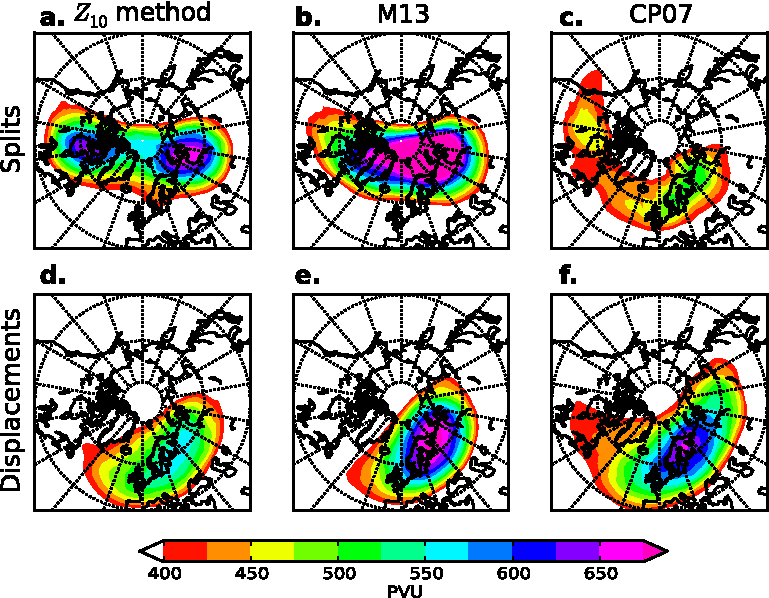
\includegraphics[width=\textwidth]{figures/chapter-moments/pv_composites_colbar_crop.pdf}
 \caption[PV composites for split and displaced vortex events.]{Composites of
   potential vorticity at the 850~K isentropic surface from the ECMWF reanalyses
   over 1958-2009. Composites are taken over the 5 days following the onset date
   of split vortex events (a,b,c) and 7 days following displaced vortex events
   (d,e,f) (the difference is due to the different timescales of these
   events). We compare the current ($Z_{10}$) method (a,b) with that of M13
   (b,e) and CP07 (c,f).}
 \label{Fig3}
 \end{figure}

 Figure \ref{Fig3} demonstrates that the $Z_{10}$ method succeeds in identifying
 displaced and split vortex events events as well as, and in some cases better
 than, the methods of M13 or CP07. When comparing the three methods, CP07 is the
 clear outlier. This is most likely because the CP07 approach employs a
 zonal-mean threshold which cannot accurately capture the extreme events (M13).

\section{Summary}

Recent research has demonstrated the need to distinguish between displaced and
split stratospheric polar vortex events, due to their different impacts on
surface weather patterns. However, current methods to identify these events are
complex or require non-standard variables. In this chapter, a new, robust method
has been developed to identify displaced and split vortex events, which requires
only geopotential height at 10~hPa. The method is briefly summarised as follows:
 \begin{enumerate}
 \item To identify the vortex region, a single contour of 10~hPa geopotential
   height is selected: the value of the zonal mean at $60^{\circ}$N.
 \item Using this contour and the geopotenial height field, the centroid
   latitude and aspect ratio are calculated, following the methodology of
   \cite{Matthewman2009}.
 \item Events are identified using a threshold criterion: Displaced events are
   identified if the centroid latitude remains equatorward $66^{\circ}$N for 7
   days or more. Split events are identified if the aspect ratio remains above
   2.4 for 7 days or more. No two events may occur within 30 days.
 \end{enumerate}

 Results using this method demonstrate that it is able to identify split and
 displaced vortex events at least as effectively as previous methods.

% ------------------- Copied from 2nd year report --------------%
\pagebreak

\begin{figure}
 \centering
 \noindent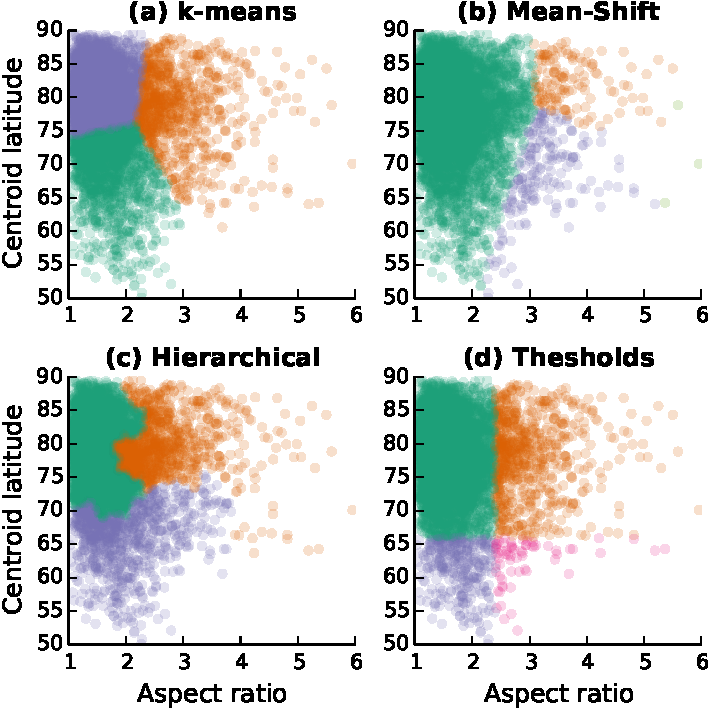
\includegraphics[width=0.7\textwidth]{figures/chapter-moments/clustering.pdf}
 \caption[Clustering algorithms applied to the moment diagnostics.]{Three
   clustering algorithms and a threshold division applied to the moment
   diagnostics in centroid latitude-aspect ratio space. For the $k$-means and
   hierarchical algorithms three clusters were specified. The mean-shift
   algorithm determined the number of clusters to be 4.}
 \label{fig:clusters}
\end{figure}


\begin{figure}
 \centering
 \noindent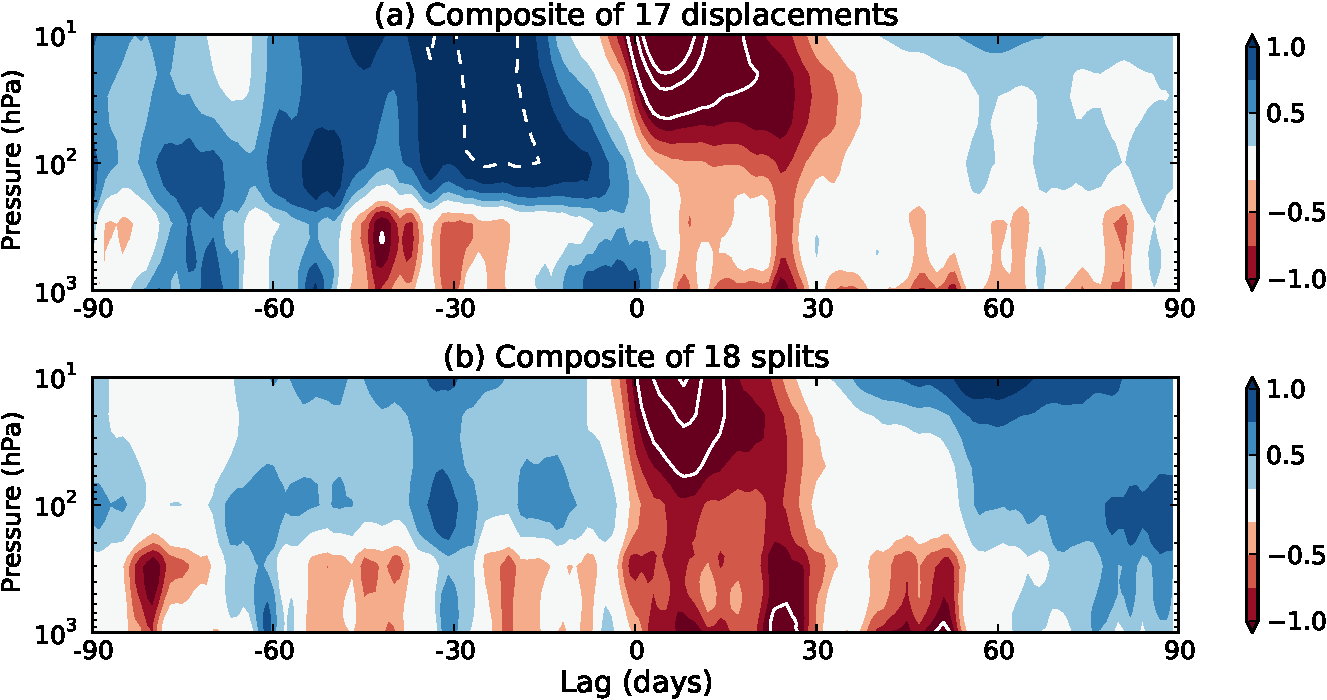
\includegraphics[width=\textwidth]{figures/chapter-moments/dripping_paint_crop.pdf}
 \caption[NAM composites for split and displaced vortex events.]{Composites of
   the time-height evolution of the NAM during (a) 17 vortex displacement events
   and (b) 18 splitting events. Lag 0 shows the onset of an event as measured at
   10 hPa. Contour intervals are 0.25 and the region between -0.25 and 0.25 is
   unshaded. Data is from the ECMWF Reanalyses 1958-2009.}
 \label{Fig3}
\end{figure}

\begin{figure}
 \centering
 \noindent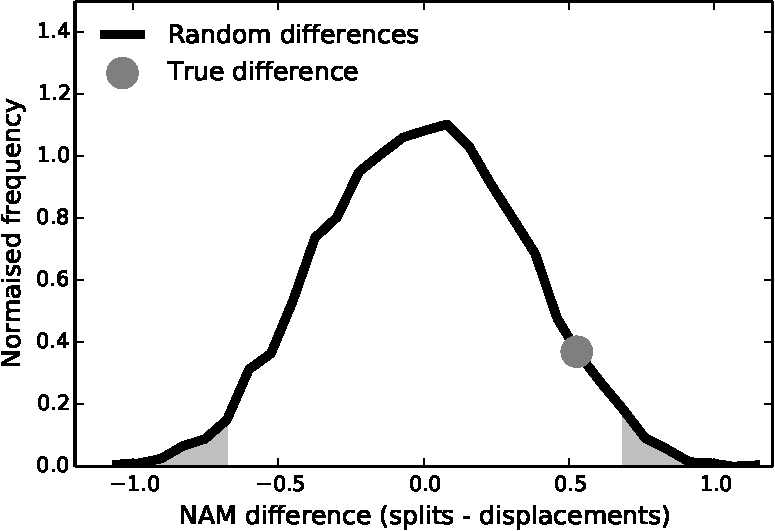
\includegraphics[width=0.7\textwidth]{figures/chapter-moments/nam_difference_sig.pdf}
 \caption[Significance of surface NAM difference following split and displaced
 vortex events.]{Distribution of 0-30 day mean NAM composite differences between
   split and displaced vortex events, formed by randomly shuffling the labels
   `split' and `displacement' between events. The 95\% significant region
   (according to a two-tailed test) is shaded and the true composite difference
   is at the 94th percentile.}
 \label{Fig3}
\end{figure}

\begin{figure}
 \centering
 \noindent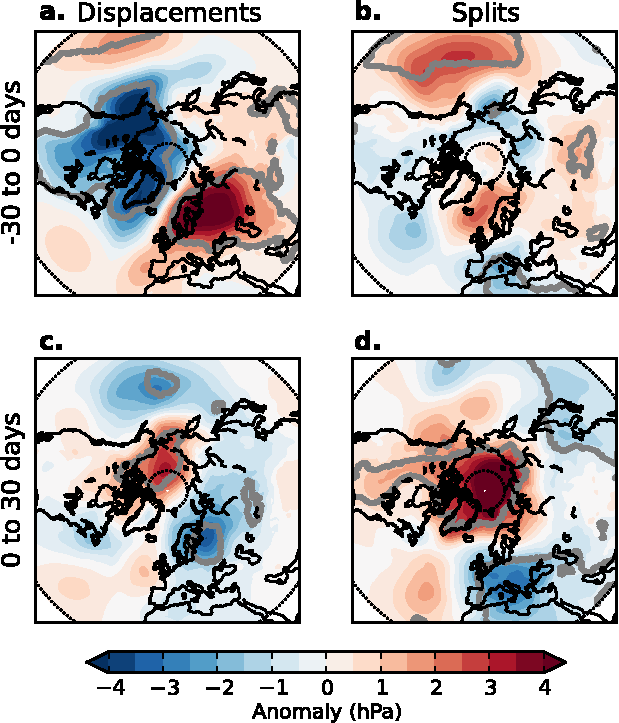
\includegraphics[width=0.7\textwidth]{figures/chapter-moments/mslp_composites_colbar_crop.pdf}
 \caption[Mean sea-level pressure composites for split and displaced vortex
 events.]{Composites of mean sea-level pressure anomalies in the 30 days before
   (a,b) and 30 days after (c,d) the onset dates of displaced (a,c) and split
   (b,d) vortex events from the $Z_{10}$ method. Data is from the ECMWF
   renalyses (1958-2009). Anomalies are calculated for each day and gridpoint
   from the climatology for that day of the year and gridpoint. Grey contours
   indicate regions of greater than 95\% statistical significance according to a
   Monte-Carlo significance test.}
 \label{Fig3}
\end{figure}


M13 found that the mean sea-level pressure (MSLP) anomalies are different before
and after displaced and split vortex events. In Figure \ref{fig:mslp_comp} we
present composites of MSLP 30 days before and 30 days following the onset dates
of displaced and split vortex events, calculated using the $Z_{10}$ method, from
the ECMWF reanalyses. Statistical significance is estimated from a Monte-Carlo
method, using $10^{5}$ composites of equal size, formed from randomly sampled
winter dates. The strongest precursor is found for displaced vortex events, with
a wave-1 pattern that is similar to the stationary wave pattern
\citep[e.g.][]{Garfinkel2008}, suggesting increased wave-1 propagation into the
stratosphere. However, the strongest anomalies following events occur after
split vortex events, with a pattern resembling the negative phase of the North
Atlantic Oscillation (though with a southern centre of action shifted towards
Europe).

The evolution of anomalies throughout the depth of the atmosphere can be
investigated through the use of annular modes \citep[e.g.][]{Baldwin2001a}. The
Northern Annular Mode (NAM) (known as the Arctic Oscillation at the surface) is
the leading mode of variability in the wintertime variability of the Northern
Hemisphere circulation. Here we use the method of \citep{Baldwin2009}, who
define the NAM as the leading empirical orthogonal function (EOF) of daily
wintertime (November-April) zonal mean geopotential height anomalies poleward of
$20^{\circ}$N. The anomalies are calculated by subtracting the seasonal cycle
which has been smoothed with a 90-day low-pass filter. The daily NAM anomalies
are then determined by projecting daily geopotential anomalies onto the leading
EOF patterns. Finally, the NAM is normalised at each level so that the entire
time series has unit variance.

Figure \ref{fig:nam_comp} presents time-height composites of NAM anomalies 90
days either side of the onset date of displaced and split vortex events. Despite
the larger stratospheric anomaly following displaced vortex events, the
tropospheric signal is larger following split vortex events (as in Figure
\ref{fig:mslp_comp}). The vertical evolution of these events also differs
greatly, with anomalies descending from the upper stratosphere over a period of
weeks for displacement events, while split vortex events are near
barotropic. This suggests an excitation of the barotropic mode, which supports
the idea of the wave resonance view of SSWs \citep{Esler2005}.

Overall, these results support the findings of M13, but use a new method to
identify split and displaced vortex events, and extend the analysis to 2009. The
fact that the results are consistent suggests the findings of M13 are robust and
highlights the importance of distinguishing split and displaced vortex events in
understanding stratosphere-troposphere coupling following SSWs.






%%% Local Variables:
%%% mode: latex
%%% TeX-master: "thesis"
%%% End:
